\documentclass{article}

\usepackage{xcolor}
\usepackage{geometry}
\geometry{a4paper, total={170mm,257mm},left=20mm, top=20mm,}

\usepackage{pgf}
\usepackage{tikz}
\usetikzlibrary{arrows,automata}

\title{Évaluation d’expressions booléennes}
\author{LAZZARI-ARMOUR Raphael et POULIQUEN Chloé}
\date{Mai 2021}

\begin{document}

\maketitle

\section*{Question 1}
\textit{
\textcolor{blue}{
\underline{Question:}
 Lire une chaîne de caractère contenant une expression arithmétique et la transformer en une liste de tokens.
}
}
\newline\newline
Pour cette première question, nous avons eu besoin de définir la structure suivante. Le but du projet étant sur les "expressions booléennes", nous avons décidé de faire une structure composé uniquement de booléen. La taille d'un booléen étant de 1 bit, cela nous fait par la même occasion économiser sur la mémoire allouée pour la liste par la suite. 

\begin{verbatim}
struct token{
  struct token* next;
  type TYPE;
  union{
    bool value;             //if TYPE is a CONSTANT, value is 'true' if '1' else 'false' if '0'
    bool bracket;           //if TYPE is a BRACKET, value is 'true' if '(' else 'false' if ')'
    bool unary;             //if TYPE is a UNARY_OP, value is 'true' if 'NON' else 'false'
    op_binary OpBinary;     //if TYPE is a BINARY_OP, value depends on enum op_binary
  }attribute;
};
typedef struct token* TokenList;
\end{verbatim}

L'appel de la fonction \textit{TokenList $string\_to\_token(char* string)$} dans le main nous permet de convertir la chaîne de caractère entrée par l'utilisateur en une liste de token. Cette fonction prends en paramètre une chaîne de caractères et retourne une liste de tokens. 

\section*{Question 2}
\textit{
\textcolor{blue}{
\underline{Question:} 
Donner un automate à pile reconnaissant le langage dont les mots sont les expressions
booléennes.
}
}
\newline\newline
Pour cette question, nous proposant un automate reconnaissant le langage par état final et par pile vide. 
Une pile qui empile '(' et dépile ')'.
\newline\newline
\underline{Règle sur les constantes '0' et '1':}
Doit contenir un opérateur binaire, unaire ou '(' avant mais pas une autre constante. Peut être suivi par un opérateur binaire ou ')' mais pas par une constante. 
\newline\newline
\underline{Règle sur les opérateurs binaires '+' , '.' , '$\Rightarrow$' et '$\Leftrightarrow$' :}
Doit contenir une constante ou ')' avant et doit contenir une constante ou '(' après. Exception pour l'opérateur ' $\Leftrightarrow$' qui doit contenir une expression booléenne complète avant. On doit donc vérifier que la pile est vide. 
\newline\newline
\underline{Règle sur l'opérateur unaire 'NON' et '(':}
Ne peut pas contenir une constante avant. L'opérateur 'NON' doit être suivi par une constante ou par l'opérateur '('. Il ne peut ainsi pas être suivi par un opérateur binaire ou par ')'. 
\newline\newline
Après étude de ces règles, on peut définir l'automate suivant. La transition $\delta$ , $\Leftrightarrow$ , $\delta$ est seulement possible si la pile est vide.
\newline
\begin{figure}[!h]
\begin{center}
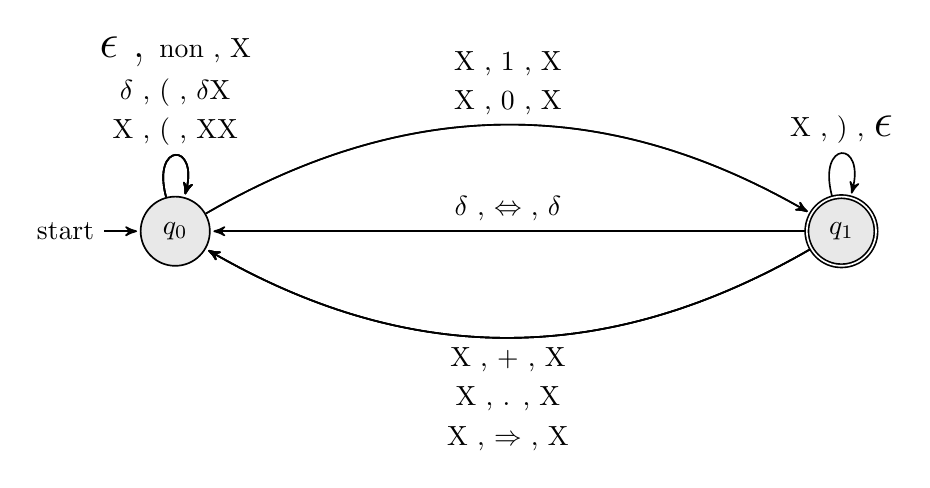
\begin{tikzpicture}[->,>=stealth',shorten >=1pt,auto,node distance=2.8cm,semithick]
  \tikzstyle{every state}=[fill={rgb:black,1;white,10}]

  \node[initial,state] 			(A)				{$q_0$};
  \node[state,accepting]         	(B) [right=8cm]	{$q_1$};

  \path	(A) 	edge	[loop above] node [above=1cm] {\LARGE{$\epsilon$} , \normalsize{non} , X} (A)
		(A)	edge	[loop above]	node [above=0.5cm] {$\delta$ , ( , $\delta$X} (A)
		(A)	edge	[loop above]	node {X , ( , XX} (A)

		(A)	edge	[bend left]	node [above=0.5cm] {X , 1 , X} (B)
		(A)	edge	[bend left]	node {X , 0 , X} (B)

		(B)	edge	[bend left]	node {X  , + , X} (A)
		(B)	edge	[bend left]	node [below=0.5cm] {X , . , X} (A)
		(B)	edge	[bend left]	node [below=1cm] {X , $\Rightarrow$ , X} (A)
		(B)	edge				node  [above] {$\delta$ , $\Leftrightarrow$ , $\delta$} (A)

		(B)	edge	[loop above]	node{X , ) , \LARGE{$\epsilon$}} (B);	

\end{tikzpicture}
\caption{Automate à pile qui reconnaît le language par état final et par pile vide.}
\end{center}
\end{figure}

\section*{Question 3}
\textit{
\textcolor{blue}{
\underline{Question:}
 Écrire une fonction en langage C qui teste si une liste de token appartient au langage ou non.
}
}

\section*{Question 4}
\textit{
\textcolor{blue}{
\underline{Question:}
À partir de la liste de tokens et en utilisant l’automate à pile, créer l’arbre représentant l’expression booléenne. Vous pouvez utiliser la fonction qui teste si la liste des tokens appartient au langage en la modifiant.
}
}

\section*{Question 5}
\textit{
\textcolor{blue}{
\underline{Question:}
Calculer la valeur de l’expression arithmétique et afficher le résultat.
}
}

\end{document}
